% !TEX TS-program = Sweave-xelatex
% see http://info.semprag.org/basics for a full description of this template
%\documentclass[linguex]{glossa}
% DO NOT FORGET TO setwd("paper/glossa/") where the Rnw file is.
\documentclass[times,linguex]{glossa}\usepackage[]{graphicx}\usepackage[]{color}
% maxwidth is the original width if it is less than linewidth
% otherwise use linewidth (to make sure the graphics do not exceed the margin)
\makeatletter
\def\maxwidth{ %
  \ifdim\Gin@nat@width>\linewidth
    \linewidth
  \else
    \Gin@nat@width
  \fi
}
\makeatother

\definecolor{fgcolor}{rgb}{0.345, 0.345, 0.345}
\newcommand{\hlnum}[1]{\textcolor[rgb]{0.686,0.059,0.569}{#1}}%
\newcommand{\hlstr}[1]{\textcolor[rgb]{0.192,0.494,0.8}{#1}}%
\newcommand{\hlcom}[1]{\textcolor[rgb]{0.678,0.584,0.686}{\textit{#1}}}%
\newcommand{\hlopt}[1]{\textcolor[rgb]{0,0,0}{#1}}%
\newcommand{\hlstd}[1]{\textcolor[rgb]{0.345,0.345,0.345}{#1}}%
\newcommand{\hlkwa}[1]{\textcolor[rgb]{0.161,0.373,0.58}{\textbf{#1}}}%
\newcommand{\hlkwb}[1]{\textcolor[rgb]{0.69,0.353,0.396}{#1}}%
\newcommand{\hlkwc}[1]{\textcolor[rgb]{0.333,0.667,0.333}{#1}}%
\newcommand{\hlkwd}[1]{\textcolor[rgb]{0.737,0.353,0.396}{\textbf{#1}}}%
\let\hlipl\hlkwb

\usepackage{framed}
\makeatletter
\newenvironment{kframe}{%
 \def\at@end@of@kframe{}%
 \ifinner\ifhmode%
  \def\at@end@of@kframe{\end{minipage}}%
  \begin{minipage}{\columnwidth}%
 \fi\fi%
 \def\FrameCommand##1{\hskip\@totalleftmargin \hskip-\fboxsep
 \colorbox{shadecolor}{##1}\hskip-\fboxsep
     % There is no \\@totalrightmargin, so:
     \hskip-\linewidth \hskip-\@totalleftmargin \hskip\columnwidth}%
 \MakeFramed {\advance\hsize-\width
   \@totalleftmargin\z@ \linewidth\hsize
   \@setminipage}}%
 {\par\unskip\endMakeFramed%
 \at@end@of@kframe}
\makeatother

\definecolor{shadecolor}{rgb}{.97, .97, .97}
\definecolor{messagecolor}{rgb}{0, 0, 0}
\definecolor{warningcolor}{rgb}{1, 0, 1}
\definecolor{errorcolor}{rgb}{1, 0, 0}
\newenvironment{knitrout}{}{} % an empty environment to be redefined in TeX

\usepackage{alltt}

% possible options: 
% [times] for Times font (default if no option is chosen)
% [cm] for Computer Modern font 
% [lucida] for Lucida font (not freely available)
% [brill] open type font, freely downloadable for non-commercial use from http://www.brill.com/about/brill-fonts; requires xetex
% [charis] for CharisSIL font, freely downloadable from http://software.sil.org/charis/
% for the Brill an CharisSIL fonts, you have to use the XeLatex typesetting engine (not pdfLatex)
% for headings, tables, captions, etc., Fira Sans is used: https://www.fontsquirrel.com/fonts/fira-sans
% [biblatex] for using biblatex (the default is natbib, do not load the natbib package in this file, it is loaded automatically via the document class glossa.cls)
% [linguex] loads the linguex example package
% !! a note on the use of linguex: in glossed examples, the third line of the example (the translation) needs to be prefixed with \glt. This is to allow a first line with the name of the language and the source of the example. See example (2) in the text for an illustration.
% !! a note on the use of bibtex: for PhD dissertations to typeset correctly in the references list, the Address field needs to contain the city (for US cities in the format "Santa Cruz, CA")

%\addbibresource{sample.bib} 
% the above line is for use with biblatex
% replace this by the name of your bib-file (extension .bib is required)
% comment out if you use natbib/bibtex

\let\B\relax %to resolve a conflict in the definition of these commands between xyling and xunicode (the latter called by fontspec, called by charis)
\let\T\relax
\usepackage{xyling} %for trees; the use of xyling with the CharisSIL font produces poor results in the branches. This problem does not arise with the packages qtree or forest.
\usepackage[linguistics]{forest} %for nice trees!


% \pdf* commands provide metadata for the PDF output. ASCII characters only!
\pdfauthor{Utku Turk \& Pavel Logacev}
\pdftitle{Agreement Attraction in Turkish}
\pdfkeywords{agreement attraction, syncretism, Turkish, bayesian, replication}

\title[Agreement Attraction in Turkish]{Agreement Attraction in Turkish\\ \bigskip \large Word count: 4720}
% Optional short title inside square brackets, for the running headers.

\author[T\"{u}rk \& Loga\v{c}ev]% short form of the author names for the running header. If no short author is given, no authors print in the headers.
{%as many authors as you like, each separated by \AND.
  \spauthor{Utku T\"{u}rk\\ 
  \institute{Bo\u{g}azi\c{c}i University}\\
  \small{%105, Bd. Raspail, 75005 Paris\\
  utku.turk@boun.edu.tr}
  }
  \AND
  \spauthor{Pavel Loga\v{c}ev \\
  \institute{Bo\u{g}azi\c{c}i University}\\
  \small{%Warmoesberg 26, 1000 Brussel\\
  pavel.logacev@boun.edu.tr}
  }%
}
\IfFileExists{upquote.sty}{\usepackage{upquote}}{}
\begin{document}

\SweaveOpts{concordance=TRUE}

\sffamily
\maketitle


\begin{abstract}
We report the results of two speeded acceptability judgment experiments in Turkish. We hypothesized an alternative explanation for agreement attraction effects in Turkish that is based on shallow processing. Our findings contradict our hypothesized form-driven processing strategy and support an account of agreement attraction based on the use of abstract linguistic features, rather than mere form.
\end{abstract}

\begin{keywords}
  agreement attraction; syncretism; Turkish; bayesian; replication
\end{keywords}

\rmfamily




\section{Introduction}

People often fail to accurately process grammatical dependencies between different parts of a sentence \citep[e.g.]{GibsonThomas:1999,PhillipsEtAl:2011}. For example, in \ref{ex:pearlmutter}, the auxiliary verb `\textit{were}' erroneously agrees with the syntactically unrelated attractor noun phrase headed by `\textit{cabinets}' instead of the agreement controller headed `\textit{key}'. Previous  studies in comprehension \citep{NicolEtAl:1997, PearlmutterGarnseyBock:1999} showed that participants found sentences like \ref{ex:pearlmutter} acceptable more often and read them faster compared to their counterparts with the singular attractor. This phenomenon, known as \textit{agreement attraction} \citep{BockMiller:1991} has been attested in a number of languages, such as in Arabic \citep{TuckerEtAl:2015}, Armenian \citep{AvetisyanEtAl:2020}, German \citep{LagoFelser:2018}, Hindi \citep{BhatiaDillon:2020}, Serbian \citep{RisticEtAl:2016}, Slovak \citep{BadeckerKuminiak:2007}, Spanish \citep{LagoEtAl:2015}, and recently in Turkish \citep{LagoEtAl:2018}.


\ex. \label{ex:pearlmutter} * The \underline{key} to the cabinets \underline{were} rusty from many years of disuse. 


\citet{LagoEtAl:2018} demonstrated that genitive possessor (such as `\textit{painters}' in `\textit{the painters' rival}') cause agreement attraction effects in Turkish. This finding appears to be at odds with \citeauthor{NicolEtAl:2016}'s (\citeyear{NicolEtAl:2016}) results, who failed to find a similar effect in English. \citet{LagoEtAl:2018} hypothesize that Turkish possessor noun phrases, unlike their English counterparts, may function as agreement attractors because Turkish genitive NPs may function as subjects of non-finite clauses in Turkish \citep{GokselKerslake:2005}. As a result, genitive NP in Turkish, but not in English, may match the subjecthood feature which may be used for cue-based retrieval of a verb's subject \citep{LewisVasishth:2005, ArnettWagers:2017}.

In this paper, we test an alternative explanation of \citeauthor{LagoEtAl:2018}'s (\citeyear{LagoEtAl:2018}) findings which is related to an instance of case syncretism in the experimental sentences in their experiment, which resulted in all subject head nouns being ambiguous between possessive and accusative case.


\section{Agreement Attraction in Turkish}

Turkish is an SOV word order language which uses case to mark arguments \citep{GokselKerslake:2005}. Case markers have different forms depending on whether or not the last sound is a vowel. In order to break vowel-vowel clusters, Turkish uses a variety of sounds as epenthetic consonants including `s,' `y,' or `n.'  For example, genitive case can surface as \textit{-nin} or as \textit{-in}, depending on the last consonant of the stem. Importantly, the forms of the possessive marker and the accusative case are identical except for the epenthetic consonant. This means that they surface as \textit{-i} in consonant-ending words, but as \textit{-si} and \textit{-ni} respectively in vowel-ending words. 


\citet{LagoEtAl:2018} present a speeded acceptability judgment study with sentences like \ref{ex:lago}, in which the number of the attractor and the verb was manipulated. The resulting 2x2 design indicated by slashes in \ref{ex:lago} consisted of two grammatical conditions, in which the verb agreed with the singular subject head noun, and two ungrammatical conditions, in which the verb carried plural agreement, and thus did not agree with the subject. In ungrammatical sentences, they found a higher percentage of `\textit{acceptable}' responses when the genitive attractor was plural than when it was singular, indicating agreement attraction. No such effect was found in grammatical sentences.


\ex. \label{ex:lago}
\gll Ressam-lar/$\emptyset$-(n)ın rakib-i atölye-den hızla uzaklaş-tı-lar/$\emptyset$.\\
painter-pl/sg-gen rival-poss workshop-abl quickly walked.away-pst-pl/sg\\
\glt `The painter's/painters' rival walked away from the workshop quickly.'


\citet{LagoEtAl:2018} hypothesized that these effects originated from how case and number information is encoded and retrieved. According to \citeauthor{LewisVasishth:2005}'s (\citeyear{LewisVasishth:2005}) cue-based retrieval model, phrases are encoded in a content-addressable memory as bundles of features called \textit{chunks} which include information like number, gender, case, and syntactic function \citep{SmithVasishth:2020}. Under \citeauthor{LagoEtAl:2018}'s (\citeyear{LagoEtAl:2018}) proposal, participants predict the number of the verb based on the chunks they formed while reading the subject. In grammatical sentences with singular verb agreement, the number prediction and the verb number match, which causes no processing difficulty. In contrast, when participants fail to find the predicted number morphology on the verb, a memory-retrieval process is initiated. This process activates the search for a chunk matching two cues: the subjecthood feature ([+SUBJECT]) and the plural feature ([+PL]). While neither of the available noun phrases matches this specification in ungrammatical agreement attraction sentences, each of the NPs headed by `\textit{painter}' and `\textit{rival}' matches one of these cues. While this partial match mostly results in participants finding the sentence ungrammatical, they may retrieve the attractor `\textit{painters}' on some trials. \citet{LagoEtAl:2018} argue that this erroneous retrieval may be facilitated by the fact that genitive case marking on the attractor because genitive NPs can function as subjects of embedded clauses in Turkish. Due to the ubiquity of genitive subjects, attractors marked with genitive case were hypothesized to be a priori more likely agreement controllers.

A potential problem with the stimuli in the \citet{LagoEtAl:2018} study is that all head nouns such as `\textit{rival}' in \ref{ex:lago} were consonant-ending and therefore locally ambiguous between possessive and accusative case \citet{GokselKerslake:2005}. Because accusative NPs cannot function as subjects in Turkish, it is possible that the agreement attraction effects found in sentences like \ref{ex:lago} are not due to the genitive attractors' association with subjecthood, but rather due to the head nouns' reduced association with subjecthood due case syncretism. We tested this hypothesis in a speeded-acceptability experiment with sentences similar to \citeauthor{LagoEtAl:2018}'s (\citeyear{LagoEtAl:2018}), but with unambiguously marked vowel-ending head nouns.


\section{The Present Study}

The present study tested predictions of the syncretism between possessive and accusative cases as an alternative explanation of the previously found agreement attraction effect in Turkish. We disambiguated between them by using vowel-ending nouns instead of consonant-ending head nouns as done in \citet{LagoEtAl:2018}. When attached to a vowel-ending noun, the possessive is realized as using \textit{-nı}, while the accusative maker would surface as \textit{-yı}. We hypothesized that if the morpho-phonological ambiguity was a key factor in agreement attraction in Turkish, resolving it should diminish the attraction effects.

\subsection{Participants} 

We recruited 118 undergraduate students to participate in the experiment in exchange for course credit. All participants were native Turkish speakers, with an average age of 20 (range: 18 -- 32). The experiment was carried out following the principles of the Declaration of Helsinki and the regulations concerning research ethics at Boğaziçi University. All participants provided informed consent before their participation.



\subsection{Materials}

We used 40 sets of sentences like \ref{ex:our_items}, in which we manipulated (i) the number of the attractor noun and (ii) the number agreement on the verb. Plural number and plural agreement were both marked with the suffix \textit{-ler/-lar}, while the singular number and singular agreement were marked by its absence. We used the experimental items from \citet{LagoEtAl:2018} as a starting point for all items. We substituted ambiguous nouns for unambiguous alternatives, and in some cases, modified other parts of the sentence for plausibility reasons.

All sentences started with a complex subject NP like `\textit{the manager's cook}' (`\textit{yöneticinin aşcısı}'), in which the genitive possessor functioned as the attractor, and the head noun carried an unambiguous possessive case marker. Because the optional plural marking is not relevant for nominals and the head noun was singular, absent of \textit{-lar}, in all conditions, sentences with plural verb agreement were ungrammatical. Moreover, the relationship between the possessor and the head noun was controlled as in \citeauthor{LagoEtAl:2018}'s (\citeyear{LagoEtAl:2018}) original study and can be paraphrased using \textit{'s} or \textit{of} in English. The distribution of the verb types matched that of the original study, with twenty unergatives, eighteen unaccusatives, and two optionally transitive verbs. Pre-verbal adverbials also consisted of 2-3 words (15 characters on average).

One example set of experimental items is in \ref{ex:our_items}. The subject phrase is marked with square brackets, and the dependency between the subject head and the matrix verb is signaled using bold-face.


\ex. \label{ex:our_items}
  \a. Plural Attractor, Ungrammatical (Plural Verb) \label{ex:expitem-plpl}\\
  \gll *[Yönetici-ler-in \textbf{aşcı-sı}] mutfak-ta sürekli \textbf{zıpla-dı-lar}\\ 
  manager-\textsc{pl}-\textsc{gen}  cook-\textsc{poss} kitchen-\textsc{loc} non-stop  jump-\textsc{pst}-\textsc{pl}.\\
  \glt `The cooks of the manager were jumping in the kitchen non-stop.'
  \b. Plural Attractor, Grammatical (Singular Verb) \label{ex:expitem-plsg} \\
  \gll [Yönetici-ler-in \textbf{aşcı-sı}] mutfak-ta sürekli \textbf{zıpla-dı}\\ 
  manager-\textsc{pl}-\textsc{gen}  cook-\textsc{poss} kitchen-\textsc{loc} non-stop  jump-\textsc{pst}.\\
  \glt `The cooks of the manager was jumping in the kitchen non-stop.'
  \b. Singular Attractor, Ungrammatical (Plural Verb) \label{ex:expitem-sgpl}\\
  \gll *[Yönetici-nin \textbf{aşcı-sı}] mutfak-ta sürekli \textbf{zıpla-dı-lar}.\\ 
  manager-\textsc{gen}  cook-\textsc{poss} kitchen-\textsc{loc} non-stop  jump-\textsc{pst}-\textsc{pl}\\
  \glt `The cook of the manager were jumping in the kitchen non-stop.'
  \b. Singular Attractor, Grammatical (Singular Verb) \label{ex:expitem-sgsg}\\
  \gll [Yönetici-nin \textbf{aşcı-sı}] mutfak-ta sürekli \textbf{zıpla-dı}. \\ 
  manager-\textsc{gen}  cook-\textsc{poss} kitchen-\textsc{loc} non-stop  jump-\textsc{pst}\\
  \glt `The cook of the manager was jumping in the kitchen non-stop.'
  

We hypothesized that the experimental sentences in \ref{ex:our_items} might elicit a simple response strategy based on verb number because all ungrammatical sentences end with a plural-agreement-bearing verb. In contrast, all grammatical sentences end with a verb that lacks a plural agreement, thus singular. As a result, some participants may resort to classifying sentence acceptability based on their last word after repeated exposure to sentences like \ref{ex:our_items}. In order to preclude such a response strategy, we designed 40 filler sentences that would render it ineffective. We included 20 grammatical sentences like \ref{ex:gram_filler} with plural and 20 ungrammatical sentences like \ref{ex:ung_filler} with a singular verb. Filler items resembled experimental sentences in that they started with a complex genitive-possessive noun phrase. In contrast to the experimental items, however, the complex NPs were the subject of an adverbial clause instead of the main sentence. In grammatical fillers like \ref{ex:gram_filler}, we have used pro-dropped subjects, which enabled us to use plural verbs without having ungrammatical sentences. 


\ex. \label{ex:fillers}
  \a. Grammatical Filler (Plural Verb) \label{ex:gram_filler}\\
  \gll [Sosyolog-un \textbf{öğrenci-si}] konuş-unca tutarsızlık açığ-a \textbf{çıkar-dı-lar}.\\ 
  sociolog-\textsc{gen}  student-\textsc{poss} speak-\textsc{nmlz} inconsistency  open-\textsc{dat} deduct-\textsc{pst}-\textsc{pl}\\
  \glt `When the student of the sociologist spoke, they revealed an inconsistency.'
  \b. Ungrammatical Filler (Singular Verb) \label{ex:ung_filler}\\
  \gll *[Dansöz-ün \textbf{koca-sı}] var-ınca kapı sakince \textbf{aç-tı}. \\
  dancer-\textsc{gen}  husband-\textsc{poss} arrive-\textsc{nmlz} door slowly  open-\textsc{pst}\\
  \glt Intended:`When the husband of the dancer came, the door opened slowly.'


\subsection{Procedure}

The experiment was run online, using the web-based platform Ibex Farm \citep{Drummond2013}. Each experimental session took approximately 25 minutes to complete. Participants provided demographic information and gave informed consent to participate in the experiment. They then proceeded to read the instructions and were given nine practice trials before the experiment began.

Each trial began with a blank screen for 600 ms, followed by a word-by-word RSVP presentation of the sentence in the center of the screen, followed by a prompt to indicate their acceptability judgment. Sentences were presented word-by-word in the center for the screen in 30 pt font size, at a rate of 400 ms per word. Participants saw a blank screen for 100 ms between each word, and to see the next item, they needed to press the 'space' key. Participants were asked to press the key 'P' to indicate that a sentence is acceptable and 'Q' to indicate that the sentence is unacceptable. They were instructed to provide judgments as quickly as possible. During the experiment, a warning message in red font appeared if they did not respond within 5,000 ms.

Participants saw 40 experimental and 40 filler sentences. Experimental sentences were distributed among four different lists according to a Latin-square design. Every participant saw one version of the experiment with a specific list and one item per condition.

\subsection{Analysis}

In order to test whether the morphological ambiguity present in the \citet{LagoEtAl:2018} sentences affected the presence or magnitude of the agreement attraction effect we analyzed the data from the present experiment together with \citeauthor{LagoEtAl:2018}'s (\citeyear{LagoEtAl:2018}) data, using the experiment as an additional factor in the analysis.
  
Prior to the analysis, we removed the data for all participants who failed to show sufficient sensitivity to the effect of grammaticality in singular attractor conditions, i.e., when no agreement attraction was expected. Specifically, we removed all participants for whom the difference in the percentage of `yes' responses between the grammatical condition \ref{ex:expitem-sgsg} and the ungrammatical condition \ref{ex:expitem-sgpl} fell below the threshold of 0.25 percentage points. We also excluded trials in which the participants missed the response deadline or gave too fast responses (below 200 ms). As a result, we excluded 10.22\% of the trials from our experiment and 2.38\% of the \citeauthor{LagoEtAl:2018}'s (\citeyear{LagoEtAl:2018}) trials. 

We analyzed responses using a Bayesian GLM assuming a Bernoulli-distributed response with a probit link function.  We used the R packages brms \citep{brms} and rstan \citep{rstan} to fit Bayesian hierarchical models \citep[e.g.]{GelmanHill:2007, NicenboimVasishth:2016}. We analyzed only experimental sentences and used (i) grammaticality of the sentence, (ii) attractor number, and (iii) presence of morphological ambiguity (i.e., experiment), as well as all their interactions as predictors. We used by-participant and by-item intercepts and slopes for all predictors. All factors were sum-coded. We have used standard priors provided by the brms package. 

In the results section, we provide posterior distributions for parameters given our data and model with 95\% credible intervals. For our models, we run 4 chains, each of which consists of 1000 warm-up iterations and 1000 sampling iterations. Data for our study, along with our analysis scripts can be found \href{https://anonymous.4open.science/r/replication_lagoetal2018-AC8C/}{here}.


\subsection{Results}

Figure \ref{fig:AverageResponses} shows the average proportions of `acceptable' responses by experimental condition for both the original experiment in \citet{LagoEtAl:2018} and our replication with unambiguous possessive marking. It shows that ungrammatical sentences with plural attractors are rated as acceptable more often (M = 0.22, SE = 0.01) than their counterparts with singular attractors (M = 0.11, SE=0.01). The magnitude of the effect (0.11) was in line with the findings reported in \citet{LagoEtAl:2018}, where the difference was 0.11. Accuracy rates for grammatical conditions were nearly equal (M = 0.93 and 0.92, SE = 0.01 and 0.01, for singular and plural attractors respectively).

\begin{figure}[hbt!]
\centering
\caption{The average percentage of acceptable responses according to the experimental conditions in our study and \citet{LagoEtAl:2018}. Error bars signal standard errors calculated following.}

\begin{knitrout}
\definecolor{shadecolor}{rgb}{0.969, 0.969, 0.969}\color{fgcolor}

{\centering 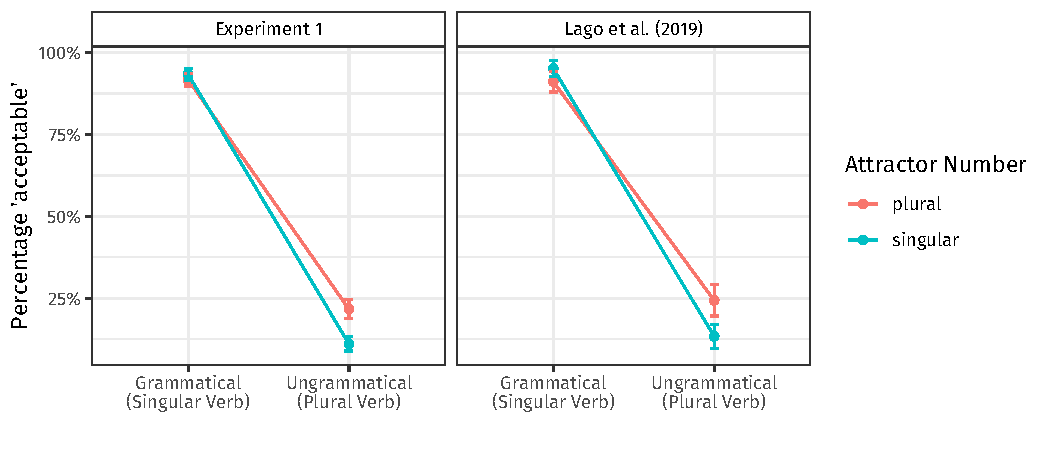
\includegraphics[width=0.9\textwidth]{figure/AverageResponses-1} 

}


\end{knitrout}

\label{fig:AverageResponses}
\end{figure}



Figure \ref{fig:ResponseModel} shows estimates and 95\% credible intervals of a Bayesian GLM with a probit link function. The main effect of grammaticality ($\hat{\beta}=3.08;$ $CI=[2.84; 3.33];$ $P(\beta<0)< .001$) indicates that, on average, participants were quite good at distinguishing between grammatical and ungrammatical sentences. Meanwhile, the negative interaction between grammaticality and attractor number ($\hat{\beta}=-0.73;$ $CI=[-1.04; -0.42];$ $P(\beta<0)> .999$) indicated a more prominent effect of attractor number in ungrammatical conditions, and thus a number agreement attraction effect. There was weak evidence for a negative three-way interaction between the presence of ambiguity, ungrammaticality, and attractor number ($\hat{\beta}=-0.27;$ $CI=[-0.77; 0.25];$ $P(\beta<0)=    .85$).


\begin{figure}[hbt!]
\centering
\caption{Estimates and 95\% credible intervals for the regression coefficients for the model of our experiment and \citet{LagoEtAl:2018}.}

\begin{knitrout}
\definecolor{shadecolor}{rgb}{0.969, 0.969, 0.969}\color{fgcolor}\begin{kframe}


{\ttfamily\noindent\color{warningcolor}{\#\# Warning in is.na(x): is.na() applied to non-(list or vector) of type 'expression'}}\end{kframe}
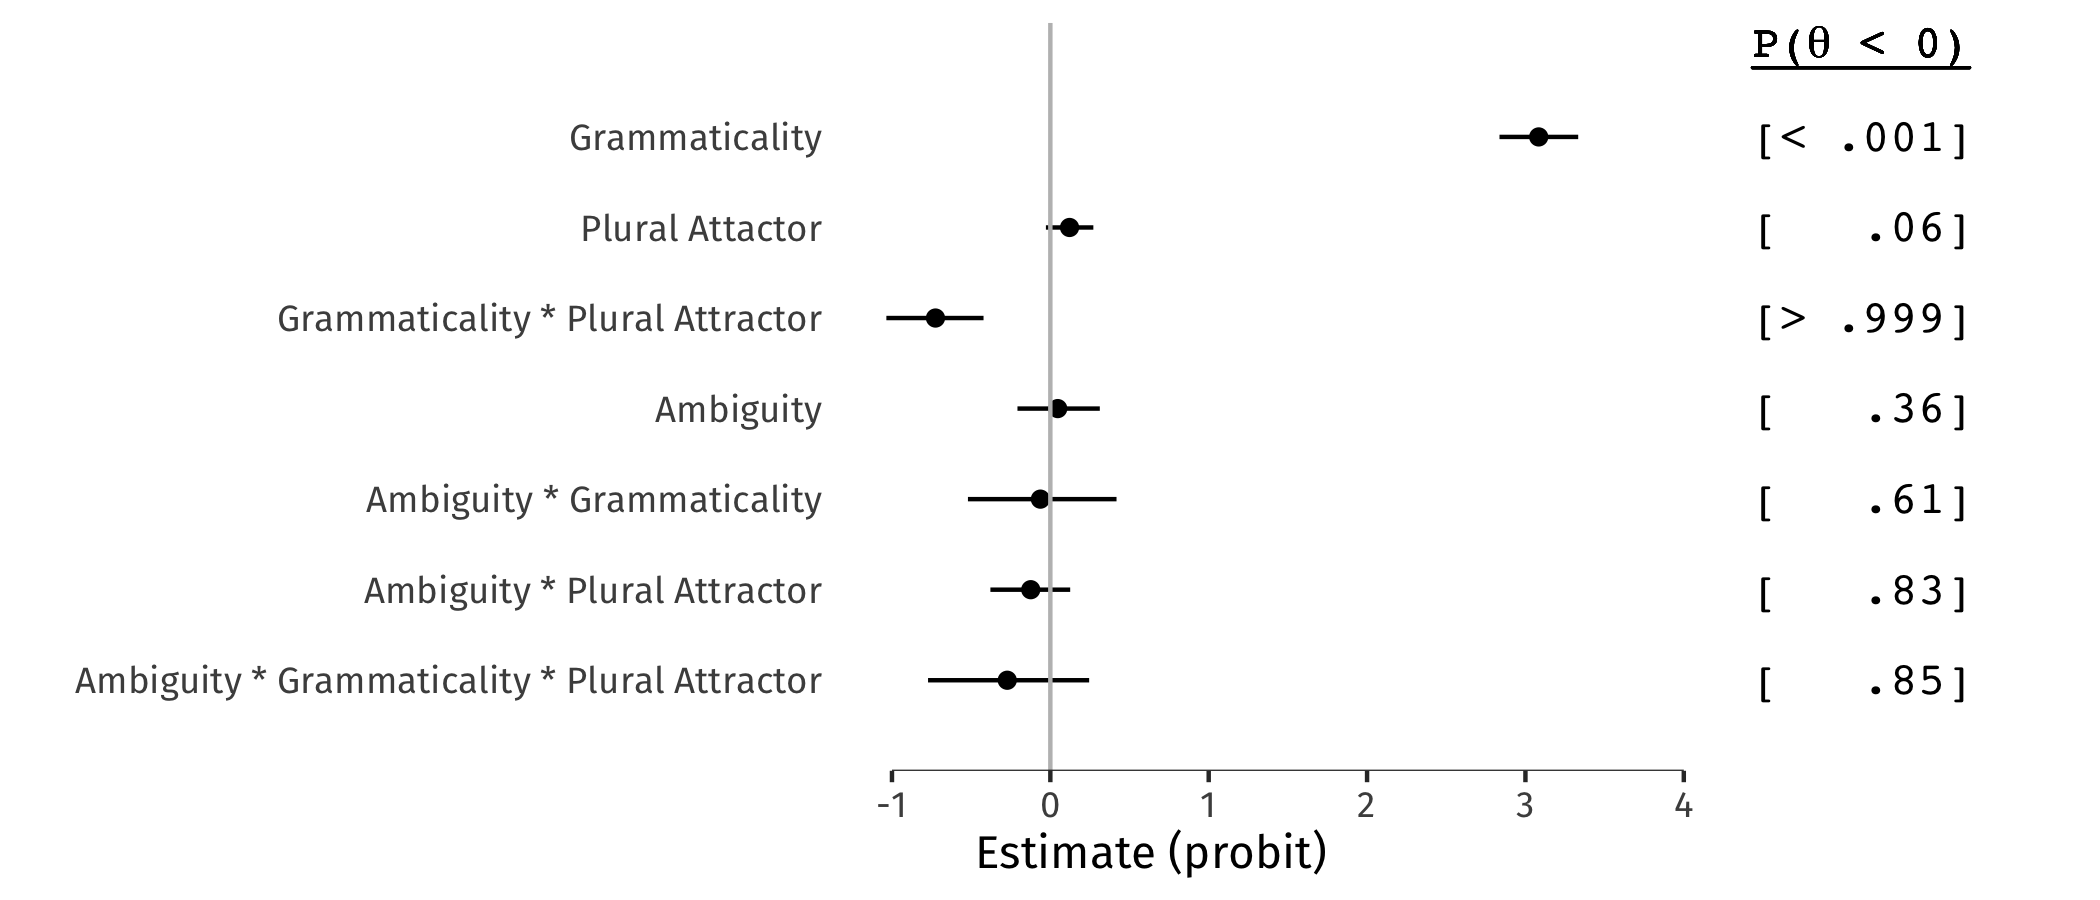
\includegraphics[width=\maxwidth]{figure/ResponseModel-1} 
\end{knitrout}

\label{fig:ResponseModel}
\end{figure}


\section{Discussion \& Conclusion}

In this paper, we re-examined the findings of \citet{LagoEtAl:2018} and investigated the effect of local case ambiguity on Turkish agreement attraction using genitive-possessive constructions in a speeded acceptability judgment experiment. The main question we asked was whether \citeauthor{LagoEtAl:2018}'s (\citeyear{LagoEtAl:2018}) findings can be explained with an alternative hypothesis. In their work, there was a possible confound in the experimental items. All head nouns were locally ambiguous between the possessive and the accusative case. We hypothesized that participants may encode the head-noun as marked with the accusative case (a non-subject case in Turkish), and thus, the retrieval of the head subject may be hindered in some trials. If Turkish agreement attraction effects resulted from this ambiguity, we should not observe any effect of plural attractor in ungrammatical sentences when the case of the head noun is disambiguated.      
  
Our experimental findings were comparable with \citet{LagoEtAl:2018} and previous agreement attraction studies. We observed that the existence of a plural attractor increased the overall error rates the participants did, and this effect was amplified even more in ungrammatical sentences. As for the effects of case ambiguity, the findings did not support our hypothesis. The findings were not conclusive on whether or not ambiguity played a role. Participants still retrieved plural attractors in ungrammatical sentences more than they did with singular attractors. 
  
Our model, where we incorporate data from both our experiment and \citet{LagoEtAl:2018}, did not show a three-way interaction between Ambiguity, Grammaticality, and Plural Attractor. This means that when the possessive marker is disambiguated agreement attraction (the interaction between Grammaticality and Plural Attractor) does not diminish in effect size. Considering the posterior distributions, we interpreted these results as pointing towards a piece of inconclusive evidence for the effect of ambiguity in agreement attraction effects. As a result, we successfully replicated the findings of \citet{LagoEtAl:2018} with disambiguated head nouns. 
  
Taken together, these results suggest (i) that Turkish agreement attraction effects are not due to a possible erroneous encoding of the possessive marker, and (ii) that local ambiguities in case, syncretism, do not play a role in agreement attraction. Participants do not rely on form-related cues in decision-making processes. These findings support an agreement attraction theory that makes use of abstract linguistic features.
  
  
  

%\printbibliography %for use with biblatex; comment out if you use natbib
\bibliography{sample} %for use with natbib; comment out if you use biblatex, and change 'sample' by the name of your bib-file


\end{document}
%%% Local Variables:
%%% mode: latex
%%% TeX-master: t
%%% TeX-engine: luatex
%%% End:
